%% -*- coding:utf-8 -*-
\chapter{Limits}

\section{Definitions}

\begin{definition}[Diagram of shape]
\label{def:diagram_of_shape}
\begin{figure}[H]
  \centering
  \begin{tikzpicture}[ele/.style={fill=black,circle,minimum
          width=.8pt,inner sep=1pt},every fit/.style={ellipse,draw,inner
          sep=-2pt}]

      % the texts

      \node at (0,0) {$I$};        
      \node at (0,3) {$C$};        

      \node[ele,label=below:$a_i^{(I)}$] (ac) at (1,0) {};    
      \node[ele,label=below:$a_j^{(I)}$] (bc) at (3,0) {};    
      \node[ele,label=above:$a_i^{(C)}$] (ad) at (1,3) {};
      \node[ele,label=above:$a_j^{(C)}$] (bd) at (3,3) {};

      \node[draw,fit= (ac) (bc),minimum width=3.5cm, minimum
        height=2cm] {} ;
      \node[draw,fit= (ad) (bd),minimum width=3.5cm, minimum
        height=2cm] {} ;

      \draw[->,thick,shorten <=2pt,shorten >=2pt] (ac) to
      node[below]{$g_{ij}^{(I)}$} (bc);
      \draw[->,thick,shorten <=2pt,shorten >=2pt] (ad) to
      node[above]{$g_{ij}^{(C)}$} (bd);
      \draw[->,thick,shorten <=2pt,shorten >=2pt] (ac) to
      node[left]{$g_i^{(C)} = F(a_i^{(I)})$} (ad);
      \draw[->,thick,shorten <=2pt,shorten >=2pt] (bc) to
      node[right]{$g_j^{(C)} = F(a_j^{(I)})$} (bd);
  \end{tikzpicture}
  \caption{Diagram of shape $F: \cat{I} \tof \cat{C}$. Objects
    $a_{i,j}^{(I)} \in \catob{I}$ are mapped to $a_{i,j}^{(C)} \in
    \catob{C}$. Morphisms $g_{ij}^{(I)} \in \cathom{I}$ are mapped to
    $g_{ij}^{(C)} \in \cathom{C}$}  
  \label{fig:diagram_of_shape}
\end{figure}

Let $\cat{I}$ and $\cat{C}$ are 2 categories. The \textit{diagram of
  shape} $\cat{I}$ in $\cat{C}$ is a \mynameref{def:functor}
(see \cref{fig:diagram_of_shape})
\[
F: \cat{I} \tof \cat{C}
\]
\end{definition}

\begin{definition}[Index category]
\label{def:indexcategory}
Category $\cat{I}$ in the \cref{def:diagram_of_shape} is called
\textit{Index category}.
\end{definition}

\subsection{Limit}

\begin{definition}[Cone]
\label{def:cone}
\begin{figure}[H]
  \centering
  \begin{tikzpicture}[ele/.style={fill=black,circle,minimum
          width=.8pt,inner sep=1pt},every fit/.style={ellipse,draw,inner
          sep=-2pt}]

      % the texts

      \node at (0,0) {$I$};        
      \node at (0,3) {$C$};        

      \node[ele,label=left:$a_i^{(I)}$] (ac) at (1.5,0) {};    
      \node[ele,label=right:$a_j^{(I)}$] (bc) at (3.5,0) {};    
      \node[ele,label=left:$a_i^{(C)}$] (ad) at (1.5,3) {};
      \node[ele,label=right:$a_j^{(C)}$] (bd) at (3.5,3) {};
      \node[ele,label=above:$c$] (d) at (2.5,5) {};

      \node[draw,fit= (ac) (bc),minimum width=4cm, minimum
        height=2cm] {} ;
      \node[draw,fit= (ad) (bd) (d),minimum width=5cm, minimum
        height=4cm] {} ;

      \draw[->,thick,shorten <=2pt,shorten >=2pt] (d) to
      node[left]{$f^{(c)}_i$} (ad);
      \draw[->,thick,shorten <=2pt,shorten >=2pt] (d) to
      node[right]{$f^{(c)}_j$} (bd);

      \draw[->,thick,shorten <=2pt,shorten >=2pt] (ac) to
      node[below]{$g_{ij}^{(I)}$} (bc);
      \draw[->,thick,shorten <=2pt,shorten >=2pt] (ad) to
      node[above]{$g_{ij}^{(C)}$} (bd);
      \draw[->,thick,shorten <=2pt,shorten >=2pt] (ac) to
      node[left]{$a_i^{(C)} = F(a_i^{(I)})$} (ad);
      \draw[->,thick,shorten <=2pt,shorten >=2pt] (bc) to
      node[right]{$a_j^{(C)} = F(a_j^{(I)})$} (bd);
  \end{tikzpicture}
  \caption{Cone $\catcone{c}{f}$} 
  \label{fig:cone}
\end{figure}
Let $F$ is a \mynameref{def:diagram_of_shape} $\cat{I}$ in $\cat{C}$.
A \textit{cone} to $F$ is an object $d \in \catob{C}$ with
\mynameref{def:morphism}s $f^{c} = \left\{f_i^{c}: c \to
a_i^{(C)}\right\}$, where $a_i^{(C)} = F(a_i^{(I)})$ 
indexed by objects from 
$\cat{I}$ (see \cref{fig:cone}). The cone is denoted as $\catcone{c}{f}$.
\end{definition}

\begin{definition}[Limit]
\label{def:limit}
\begin{figure}[H]
  \centering
  \begin{tikzpicture}[ele/.style={fill=black,circle,minimum
          width=.8pt,inner sep=1pt},every fit/.style={ellipse,draw,inner
          sep=-2pt}]

      % the texts

      \node at (0,0) {$I$};        
      \node at (0,7) {$C$};        

      \node[ele,label=left:$a_i^{(I)}$] (ac) at (1.5,0) {};    
      \node[ele,label=right:$a_j^{(I)}$] (bc) at (5.5,0) {};    
      \node[ele,label=left:$a_i^{(C)}$] (ad) at (1.5,3) {};
      \node[ele,label=right:$a_j^{(C)}$] (bd) at (5.5,3) {};
      \node[ele,label=above:$c$] (d) at (3.5,7) {};
      \node[ele,label=below:$l$] (l) at (3.5,5) {};

      \node[draw,fit= (ac) (bc),minimum width=6cm, minimum
        height=2.5cm] {} ;
      \node[draw,fit= (ad) (bd) (d) (l),minimum width=5cm, minimum
        height=5cm] {} ;

      \draw[->,thick,shorten <=2pt,shorten >=2pt] (d) to
      node[right]{$u$} (l);

      \draw[->,thick,shorten <=2pt,shorten >=2pt] (d) to
      node[left]{$f^{(c)}_i$} (ad);
      \draw[->,thick,shorten <=2pt,shorten >=2pt] (d) to
      node[right]{$f^{(c)}_j$} (bd);
      \draw[->,thick,shorten <=2pt,shorten >=2pt] (l) to
      node[right]{$f^{(l)}_i$} (ad);
      \draw[->,thick,shorten <=2pt,shorten >=2pt] (l) to
      node[left]{$f^{(l)}_j$} (bd);

      \draw[->,thick,shorten <=2pt,shorten >=2pt] (ac) to
      node[below]{$g_{ij}^{(I)}$} (bc);
      \draw[->,thick,shorten <=2pt,shorten >=2pt] (ad) to
      node[below]{$g_{ij}^{(C)}$} (bd);
      \draw[->,thick,shorten <=2pt,shorten >=2pt] (ac) to
      node[left]{$a_i^{(C)} = F(a_i^{(I)})$} (ad);
      \draw[->,thick,shorten <=2pt,shorten >=2pt] (bc) to
      node[right]{$a_j^{(C)} = F(a_j^{(I)})$} (bd);
  \end{tikzpicture}
  \caption{Limit $\catcone{l}{f}$} 
  \label{fig:limit}
\end{figure}
\textit{Limit} of \mynameref{def:diagram_of_shape} $F: \cat{I} \tof
\cat{C}$ is a \mynameref{def:cone} $\catcone{l}{f}$ to $F$ such that for 
any other $\catcone{c}{f}$ to $F$ exists an unique morphism $u : c \to l$
such that  $\forall a_i^{(I)} \in \catob{I}$ $f_i^{(l)} \circ u =
f_i^{(c)}$ i.e. diagram shown on \cref{fig:limit} commutes.
\end{definition}

If we have 2 objects from $\cat{C}$ ($c_1, c_2 \in \catob{C}$) then we can have a lot of
morphisms between the objects which form a set:
$\catmset[C]{c_1}{c_2}$. There is a subset of $\catmset[C]{c_1}{c_2}$
that can be 
called as cone's morphisms.
\begin{definition}[Morphisms of cones]
\begin{figure}
  \centering
  \begin{tikzpicture}[ele/.style={fill=black,circle,minimum
          width=.8pt,inner sep=1pt},every fit/.style={ellipse,draw,inner
          sep=-2pt}]

      % the texts

      \node at (0,0) {$I$};        
      \node at (0,7) {$C$};        

      \node[ele,label=left:$a_i^{(I)}$] (ac) at (1.5,0) {};    
      \node[ele,label=right:$a_j^{(I)}$] (bc) at (5.5,0) {};    
      \node[ele,label=left:$a_i^{(C)}$] (ad) at (1.5,3) {};
      \node[ele,label=right:$a_j^{(C)}$] (bd) at (5.5,3) {};
      \node[ele,label=above:$c_1$] (d) at (3.5,7) {};
      \node[ele,label=below:$c_2$] (l) at (3.5,5) {};

      \node[draw,fit= (ac) (bc),minimum width=6cm, minimum
        height=2.5cm] {} ;
      \node[draw,fit= (ad) (bd) (d) (l),minimum width=5cm, minimum
        height=5cm] {} ;

      \draw[->,thick,shorten <=2pt,shorten >=2pt] (d) to
      node[right]{$m$} (l);

      \draw[->,thick,shorten <=2pt,shorten >=2pt] (d) to
      node[left]{$f^{(c_1)}_i$} (ad);
      \draw[->,thick,shorten <=2pt,shorten >=2pt] (d) to
      node[right]{$f^{(c_1)}_j$} (bd);
      \draw[->,thick,shorten <=2pt,shorten >=2pt] (l) to
      node[right]{$f^{(c_2)}_i$} (ad);
      \draw[->,thick,shorten <=2pt,shorten >=2pt] (l) to
      node[left]{$f^{(c_2)}_j$} (bd);

      \draw[->,thick,shorten <=2pt,shorten >=2pt] (ac) to
      node[below]{$g_{ij}^{(I)}$} (bc);
      \draw[->,thick,shorten <=2pt,shorten >=2pt] (ad) to
      node[below]{$g_{ij}^{(C)}$} (bd);
      \draw[->,thick,shorten <=2pt,shorten >=2pt] (ac) to
      node[left]{$a_i^{(C)} = F(a_i^{(I)})$} (ad);
      \draw[->,thick,shorten <=2pt,shorten >=2pt] (bc) to
      node[right]{$a_j^{(C)} = F(a_j^{(I)})$} (bd);
  \end{tikzpicture}
  \caption{Morphism $m$ between 2 cones $\catcone{c_1}{f}$ and $\catcone{c_2}{f}$} 
  \label{fig:conesmorphism}
\end{figure}
Let $c_1, c_2 \in \catob{C}$ are 2 objects from category $\cat{C}$ and 
$\catcone{c_1}{f}, \catcone{c_2}{f}$ are 2 \mynameref{def:cone}s.
The morphism $m \in \catmset[C]{c_1}{c_2}$ is called as morphism of
cones if $\forall i$
\[
f_i^{(c_1)} = f_i^{(c_2)} \circ m, 
\]
i.e. the morphisms in \cref{fig:conesmorphism} commute.
\end{definition}

\begin{definition}[Category of cones to $F$]
\label{def:category_of_cones}
Let $F$ is a \mynameref{def:diagram_of_shape} $\cat{I}$ in $\cat{C}$.

TBD

The category of \mynameref{def:cone}s is denoted as $\Delta \downarrow
F$ \cite{wiki:cone} 
\end{definition}

\begin{remark}[Category of cones to $F$]
\label{rem:category_of_cones}
Let $F$ is a \mynameref{def:diagram_of_shape} $\cat{I}$ in $\cat{C}$
and $\Delta \downarrow F$ is the \mynameref{def:category_of_cones}.
Then \mynameref{def:limit} is \mynameref{def:terminal_object} in the
category.
\end{remark}

\subsection{Colimit}

\begin{definition}[Cocone]
\label{def:cocone}
\begin{figure}[H]
  \centering
  \begin{tikzpicture}[ele/.style={fill=black,circle,minimum
          width=.8pt,inner sep=1pt},every fit/.style={ellipse,draw,inner
          sep=-2pt}]

      % the texts

      \node at (0,0) {$I$};        
      \node at (0,3) {$C$};        

      \node[ele,label=left:$a_i^{(I)}$] (ac) at (1.5,0) {};    
      \node[ele,label=right:$a_j^{(I)}$] (bc) at (3.5,0) {};    
      \node[ele,label=left:$a_i^{(C)}$] (ad) at (1.5,3) {};
      \node[ele,label=right:$a_j^{(C)}$] (bd) at (3.5,3) {};
      \node[ele,label=above:$c$] (d) at (2.5,5) {};

      \node[draw,fit= (ac) (bc),minimum width=4cm, minimum
        height=2cm] {} ;
      \node[draw,fit= (ad) (bd) (d),minimum width=5cm, minimum
        height=4cm] {} ;

      \draw[->,thick,shorten <=2pt,shorten >=2pt] (ad) to
      node[left]{$f^{(c)}_i$} (d);
      \draw[->,thick,shorten <=2pt,shorten >=2pt] (bd) to
      node[right]{$f^{(c)}_j$} (d);

      \draw[->,thick,shorten <=2pt,shorten >=2pt] (ac) to
      node[below]{$g_{ij}^{(I)}$} (bc);
      \draw[->,thick,shorten <=2pt,shorten >=2pt] (ad) to
      node[above]{$g_{ij}^{(C)}$} (bd);
      \draw[->,thick,shorten <=2pt,shorten >=2pt] (ac) to
      node[left]{$a_i^{(C)} = F(a_i^{(I)})$} (ad);
      \draw[->,thick,shorten <=2pt,shorten >=2pt] (bc) to
      node[right]{$a_j^{(C)} = F(a_j^{(I)})$} (bd);
  \end{tikzpicture}
  \caption{Co-cone $\catcocone{c}{f}$} 
  \label{fig:cocone}
\end{figure}
Let $F$ is a \mynameref{def:diagram_of_shape} $\cat{I}$ in $\cat{C}$.
A \textit{co-cone} to $F$ is an object $d \in \catob{C}$ with
\mynameref{def:morphism}s $f^{c} = \left\{f_i^{c}:
a_i^{(C)} \to c \right\}$, where $a_i^{(C)} = F(a_i^{(I)})$ 
indexed by objects from 
$\cat{I}$ (see \cref{fig:cocone}). The co-cone is denoted as
$\catcocone{c}{f}$. 
\end{definition}

\begin{definition}[Colimit]
\label{def:colimit}
\begin{figure}[H]
  \centering
  \begin{tikzpicture}[ele/.style={fill=black,circle,minimum
          width=.8pt,inner sep=1pt},every fit/.style={ellipse,draw,inner
          sep=-2pt}]

      % the texts

      \node at (0,0) {$I$};        
      \node at (0,7) {$C$};        

      \node[ele,label=left:$a_i^{(I)}$] (ac) at (1.5,0) {};    
      \node[ele,label=right:$a_j^{(I)}$] (bc) at (5.5,0) {};    
      \node[ele,label=left:$a_i^{(C)}$] (ad) at (1.5,3) {};
      \node[ele,label=right:$a_j^{(C)}$] (bd) at (5.5,3) {};
      \node[ele,label=above:$c$] (d) at (3.5,7) {};
      \node[ele,label=below:$l$] (l) at (3.5,5) {};

      \node[draw,fit= (ac) (bc),minimum width=6cm, minimum
        height=2.5cm] {} ;
      \node[draw,fit= (ad) (bd) (d) (l),minimum width=5cm, minimum
        height=5cm] {} ;

      \draw[->,thick,shorten <=2pt,shorten >=2pt] (l) to
      node[right]{$u$} (d);

      \draw[->,thick,shorten <=2pt,shorten >=2pt] (ad) to
      node[left]{$f^{(c)}_i$} (d);
      \draw[->,thick,shorten <=2pt,shorten >=2pt] (bd) to
      node[right]{$f^{(c)}_j$} (d);
      \draw[->,thick,shorten <=2pt,shorten >=2pt] (ad) to
      node[right]{$f^{(l)}_i$} (l);
      \draw[->,thick,shorten <=2pt,shorten >=2pt] (bd) to
      node[left]{$f^{(l)}_j$} (l);

      \draw[->,thick,shorten <=2pt,shorten >=2pt] (ac) to
      node[below]{$g_{ij}^{(I)}$} (bc);
      \draw[->,thick,shorten <=2pt,shorten >=2pt] (ad) to
      node[below]{$g_{ij}^{(C)}$} (bd);
      \draw[->,thick,shorten <=2pt,shorten >=2pt] (ac) to
      node[left]{$a_i^{(C)} = F(a_i^{(I)})$} (ad);
      \draw[->,thick,shorten <=2pt,shorten >=2pt] (bc) to
      node[right]{$a_j^{(C)} = F(a_j^{(I)})$} (bd);
  \end{tikzpicture}
  \caption{Co-Limit $\catcocone{l}{f}$} 
  \label{fig:colimit}
\end{figure}
\textit{Co-Limit} of \mynameref{def:diagram_of_shape} $F: \cat{I} \tof
\cat{C}$ is a \mynameref{def:cocone} $\catcocone{l}{f}$ to $F$ such that for 
any other $\catcocone{c}{f}$ to $F$ exists an unique morphism $u : l \to c$
such that  $\forall a_i^{(I)} \in \catob{I}$ $u \circ f_i^{(c)} =
f_i^{(l)}$ i.e. diagram shown on \cref{fig:colimit} commutes.
\end{definition}

\begin{definition}[Category of co-cones from $F$]
\label{def:category_of_cocones}
Let $F$ is a \mynameref{def:diagram_of_shape} $\cat{I}$ in $\cat{C}$.

TBD

The category of \mynameref{def:cocone}s is denoted as $F \downarrow
\Delta$ \cite{wiki:cone}  
\end{definition}


\begin{remark}[Category of co-cones]
\label{rem:category_of_cocones}
Let $F$ is a \mynameref{def:diagram_of_shape} $\cat{I}$ in $\cat{C}$
and $F \downarrow \Delta$ is the \mynameref{def:category_of_cocones}.
Then \mynameref{def:colimit} is \mynameref{def:initial_object} in the
category. 
\end{remark}

\section{Cone as natural transformation}
The \mynameref{def:cone} can be considered as a \mynameref{def:nt}.
There are 2 functors between categories $\cat{I}$ and 
$\cat{C}$. The first one is the \mynameref{def:diagram_of_shape} $F:
\cat{I} \tof \cat{C}$. The second one is the 
\mynameref{def:const_functor}: 
$\Delta_c: \cat{I} \tof \cat{C}$. The
\mynameref{def:nt} $\Delta_c
\tont F$, by the definition, is the set of \mynameref{def:morphism}s from $\cat{C}$ with
additional relations that are same as conditions defined for
the \mynameref{def:cone} $\catcone{c}{f}$. Therefore we can consider
the \mynameref{def:cone} as a \mynameref{def:nt}. 

\section{Categorical constructions as limits}

Different choice for category $\cat{I}$ gives different types of
limits. There are several examples of such constructions below

The empty category will give us the terminal object. The
\mynameref{def:discrete_category} with 2 elements produces
\mynameref{def:product} as the \mynameref{def:limit}.

\subsection{Initial and terminal objects}

If we choose \mynameref{def:empty_category} as the
\mynameref{def:indexcategory} 
(see \cref{fig:initial_terminal_object_index_category})
then we can get
\mynameref{def:terminal_object} as \mynameref{def:limit} and
\mynameref{def:initial_object} as \mynameref{def:colimit}. 

\begin{figure}[H]
  \centering
  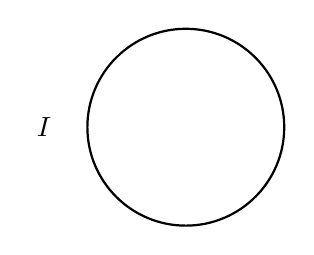
\begin{tikzpicture}[ele/.style={fill=black,circle,minimum
          width=.8pt,inner sep=1pt},every fit/.style={ellipse,draw,inner
          sep=-2pt}]

      % the texts

      \node at (0,0) {$I$};        
      \node [draw, thick, circle, minimum width=2.5cm]  at (1.8,0) {};

  \end{tikzpicture}
  \caption{Index category $I$ for initial and terminal objects. The
    category is empty} 
  \label{fig:initial_terminal_object_index_category}
\end{figure}

\begin{example}[Limit][Terminal object]
\index{Terminal object!Limit example}
Lets choose \mynameref{def:empty_category} as the
\mynameref{def:indexcategory} $\cat{I}$. 
\begin{figure}[H]
  \centering
  \begin{tikzpicture}[ele/.style={fill=black,circle,minimum
          width=.8pt,inner sep=1pt},every fit/.style={ellipse,draw,inner
          sep=-2pt}]

      % the texts

      \node at (0,0) {$I$};        
      \node at (0,3.5) {$C$};        

      \node[ele,label=above:$c$] (d) at (1.8,3.5) {};
      \node[ele,label=below:$t$] (l) at (1.8,2.5) {};

      \node [draw, thick, circle, minimum width=2.5cm]  at (1.8,0) {};
      \node[draw,fit= (d) (l),minimum width=2.5cm, minimum
        height=2.5cm] {} ;

      \draw[->,thick,shorten <=2pt,shorten >=2pt] (d) to
      node[right]{$u$} (l);

  \end{tikzpicture}
  \caption{Terminal object $t$ as a limit} 
  \label{fig:limit_terminal_object}
\end{figure}
The \mynameref{def:cone} consists from the apex $c$ only (see
\cref{fig:limit_terminal_object}). 
The \mynameref{def:limit}
will be \mynameref{def:terminal_object} in the category $\cat{C}$.
\end{example}

\begin{example}[Colimit][Initial object]
\index{Initial object!Colimit example}
Lets choose \mynameref{def:empty_category} as the
\mynameref{def:indexcategory} $\cat{I}$. 
\begin{figure}[H]
  \centering
  \begin{tikzpicture}[ele/.style={fill=black,circle,minimum
          width=.8pt,inner sep=1pt},every fit/.style={ellipse,draw,inner
          sep=-2pt}]

      % the texts

      \node at (0,0) {$I$};        
      \node at (0,3.5) {$C$};        

      \node[ele,label=above:$c$] (d) at (1.8,3.5) {};
      \node[ele,label=below:$i$] (l) at (1.8,2.5) {};

      \node [draw, thick, circle, minimum width=2.5cm]  at (1.8,0) {};
      \node[draw,fit= (d) (l),minimum width=2.5cm, minimum
        height=2.5cm] {} ;

      \draw[->,thick,shorten <=2pt,shorten >=2pt] (l) to
      node[right]{$u$} (d);

  \end{tikzpicture}
  \caption{Initial object $i$ as a colimit} 
  \label{fig:colimit_initial_object}
\end{figure}
The \mynameref{def:cocone} consists from the apex $c$ only (see
\cref{fig:colimit_initial_object}). 
The \mynameref{def:colimit}
will be \mynameref{def:initial_object} in the category $\cat{C}$. 
\end{example}

\subsection{Product and sum}

If choose \mynameref{def:discrete_category} with 2 objects as the
\mynameref{def:indexcategory} (see
\cref{fig:limit_product_index_category}) then we can get
\mynameref{def:product} 
as \mynameref{def:limit} and \mynameref{def:sum} as
\mynameref{def:colimit}. 

\begin{figure}[H]
  \centering
  \begin{tikzpicture}[ele/.style={fill=black,circle,minimum
          width=.8pt,inner sep=1pt},every fit/.style={ellipse,draw,inner
          sep=-2pt}]

      % the texts

      \node at (0,0) {$I$};        

      \node[ele,label=left:$a^{(I)}$] (a) at (2,0) {};    
      \node[ele,label=right:$b^{(I)}$] (b) at (4,0) {};    

      \draw (a) to [out=-45,in=-135,looseness=20] node[below]
            {$\idm{a^{(I)}}$} (a); 
      \draw (b) to [out=-45,in=-135,looseness=20] node[below]
            {$\idm{b^{(I)}}$} (b);


      \node[draw,fit= (a) (b),minimum width=5cm, minimum
        height=2.5cm] {} ;
  \end{tikzpicture}
  \caption{Index category $I$ for product and sum. It
    consists of 2 objects $a^{(I)}, b^{(I)}$ and 2 trivial (identity)
    morphisms $\idm{a^{(I)}}, \idm{b^{(I)}}$}   
  \label{fig:limit_product_index_category}
\end{figure}

\begin{example}[Limit][Product]
\index{Product!Limit example}
Lets choose \mynameref{def:discrete_category} with 2 objects as the
\mynameref{def:indexcategory} $\cat{I}$. 
\begin{figure}[H]
  \centering
  \begin{tikzpicture}[ele/.style={fill=black,circle,minimum
          width=.8pt,inner sep=1pt},every fit/.style={ellipse,draw,inner
          sep=-2pt}]

      % the texts

      \node at (0,0) {$I$};        
      \node at (0,7) {$C$};        

      \node[ele,label=left:$a^{(I)}$] (ac) at (1.5,0) {};    
      \node[ele,label=right:$b^{(I)}$] (bc) at (5.5,0) {};    
      \node[ele,label=left:$a$] (ad) at (1.5,3) {};
      \node[ele,label=right:$b$] (bd) at (5.5,3) {};
      \node[ele,label=above:$c$] (d) at (3.5,7) {};
      \node[ele,label=below:$a \times b$] (l) at (3.5,4) {};

      \node[draw,fit= (ac) (bc),minimum width=6cm, minimum
        height=2.5cm] {} ;
      \node[draw,fit= (ad) (bd) (d) (l),minimum width=7cm, minimum
        height=7cm] {} ;

      \draw[->,thick,shorten <=2pt,shorten >=2pt] (d) to
      node[right]{$u$} (l);

      \draw[->,thick,shorten <=2pt,shorten >=2pt] (d) to
      node[left]{$f^{(c)}_a$} (ad);
      \draw[->,thick,shorten <=2pt,shorten >=2pt] (d) to
      node[right]{$f^{(c)}_b$} (bd);
      \draw[->,thick,shorten <=2pt,shorten >=2pt] (l) to
      node[above]{$f^{(l)}_a$} (ad);
      \draw[->,thick,shorten <=2pt,shorten >=2pt] (l) to
      node[above]{$f^{(l)}_b$} (bd);

      \draw[->,thick,shorten <=2pt,shorten >=2pt] (ac) to
      node[left]{$a = F(a^{(I)})$} (ad);
      \draw[->,thick,shorten <=2pt,shorten >=2pt] (bc) to
      node[right]{$b = F(b^{(I)})$} (bd);
  \end{tikzpicture}
  \caption{Product as a limit} 
  \label{fig:limit_product}
\end{figure}
The 
\mynameref{def:diagram_of_shape} $F$ gives us the mapping into 2
objects in the category $\cat{C}$ (see \cref{fig:limit_product}). The
\mynameref{def:limit} of the 
\mynameref{def:diagram_of_shape} is the \mynameref{def:product} of the
2 objects in the category $\cat{C}$.
\end{example}

\begin{example}[Colimit][Sum]
\index{Sum!Colimit example}
Lets choose \mynameref{def:discrete_category} with 2 objects as the
\mynameref{def:indexcategory} $\cat{I}$. 
\begin{figure}[H]
  \centering
  \begin{tikzpicture}[ele/.style={fill=black,circle,minimum
          width=.8pt,inner sep=1pt},every fit/.style={ellipse,draw,inner
          sep=-2pt}]

      % the texts

      \node at (0,0) {$I$};        
      \node at (0,7) {$C$};        

      \node[ele,label=left:$a^{(I)}$] (ac) at (1.5,0) {};    
      \node[ele,label=right:$b^{(I)}$] (bc) at (5.5,0) {};    
      \node[ele,label=left:$a$] (ad) at (1.5,3) {};
      \node[ele,label=right:$b$] (bd) at (5.5,3) {};
      \node[ele,label=above:$c$] (d) at (3.5,7) {};
      \node[ele,label=below:$a \oplus b$] (l) at (3.5,4) {};

      \node[draw,fit= (ac) (bc),minimum width=6cm, minimum
        height=2.5cm] {} ;
      \node[draw,fit= (ad) (bd) (d) (l),minimum width=7cm, minimum
        height=7cm] {} ;

      \draw[->,thick,shorten <=2pt,shorten >=2pt] (l) to
      node[right]{$u$} (d);

      \draw[->,thick,shorten <=2pt,shorten >=2pt] (ad) to
      node[left]{$f^{(c)}_a$} (d);
      \draw[->,thick,shorten <=2pt,shorten >=2pt] (bd) to
      node[right]{$f^{(c)}_b$} (d);
      \draw[->,thick,shorten <=2pt,shorten >=2pt] (ad) to
      node[above]{$f^{(l)}_a$} (l);
      \draw[->,thick,shorten <=2pt,shorten >=2pt] (bd) to
      node[above]{$f^{(l)}_b$} (l);

      \draw[->,thick,shorten <=2pt,shorten >=2pt] (ac) to
      node[left]{$a = F(a^{(I)})$} (ad);
      \draw[->,thick,shorten <=2pt,shorten >=2pt] (bc) to
      node[right]{$b = F(b^{(I)})$} (bd);
  \end{tikzpicture}
  \caption{Sum as a colimit} 
  \label{fig:colimit_sum}
\end{figure}
The 
\mynameref{def:diagram_of_shape} $F$ gives us the mapping into 2
objects in the category $\cat{C}$ (see \cref{fig:colimit_sum}). The
\mynameref{def:colimit} of the 
\mynameref{def:diagram_of_shape} is the \mynameref{def:sum} of the
2 objects in the category $\cat{C}$.
\end{example}

\subsection{Equalizer}

If choose a \mynameref{def:category} with 2 objects as the
\mynameref{def:indexcategory} (see
\cref{fig:limit_equlizer_index_category}) and 2 \mynameref{def:morphism}s
connecting one object with another then we can get equalizer 
as \mynameref{def:limit}. 

\begin{figure}[H]
  \centering
  \begin{tikzpicture}[ele/.style={fill=black,circle,minimum
          width=.8pt,inner sep=1pt},every fit/.style={ellipse,draw,inner
          sep=-2pt}]

      % the texts

      \node at (0,0) {$I$};        

      \node[ele,label=left:$a^{(I)}$] (a) at (2,0) {};    
      \node[ele,label=right:$b^{(I)}$] (b) at (4,0) {};    

      \draw[->,thick,shorten <=2pt,shorten >=2pt] (a) to
           [out=45,in=135,looseness=1] node[above] {$f^{(I)}$} (b); 
      \draw[->,thick,shorten <=2pt,shorten >=2pt] (a) to
           [out=-45,in=-135,looseness=1] node[above] {$g^{(I)}$} (b); 


      \draw (a) to [out=-45,in=-135,looseness=20] node[below]
            {$\idm{a^{(I)}}$} (a); 
      \draw (b) to [out=-45,in=-135,looseness=20] node[below]
            {$\idm{b^{(I)}}$} (b);


      \node[draw,fit= (a) (b),minimum width=5cm, minimum
        height=2.5cm] {} ;
  \end{tikzpicture}
  \caption{Index category $I$ for equalizer. It
    consists of 2 objects $a^{(I)}, b^{(I)}$, 2 trivial (identity)
    morphisms $\idm{a^{(I)}}, \idm{b^{(I)}}$ and 2 additional morphisms
   $f^{(I)}, g^{(I)} \in \catmset[I]{a^{(I)}}{b^{(I)}}$}   
  \label{fig:limit_equlizer_index_category}
\end{figure}

\begin{definition}[Equalizer]
\label{def:equalizer}
Lets choose a \mynameref{def:category} with 2 objects $a^{(I)},
b^{(I)}$ and 2 additional morphisms
   $f^{(I)}, g^{(I)} \in \catmset[I]{a^{(I)}}{b^{(I)}}$ as the
\mynameref{def:indexcategory} $\cat{I}$ (see
\cref{fig:limit_equlizer_index_category}).    
\begin{figure}[H]
  \centering
  \begin{tikzpicture}[ele/.style={fill=black,circle,minimum
          width=.8pt,inner sep=1pt},every fit/.style={ellipse,draw,inner
          sep=-2pt}]

      % the texts

      \node at (0,0) {$I$};        
      \node at (0,7) {$C$};        

      \node[ele,label=left:$a$] (a) at (1.5,3) {};
      \node[ele,label=right:$b$] (b) at (5.5,3) {};
      \node[ele,label=above:$c$] (c) at (3.5,7) {};
      \node[ele,label=below:$eq$] (l) at (3.5,4.5) {};


      \draw[->,thick,shorten <=2pt,shorten >=2pt] (a) to
           [out=45,in=135,looseness=0.5] node[above] {$f$} (b); 
      \draw[->,thick,shorten <=2pt,shorten >=2pt] (a) to
           [out=-45,in=-135,looseness=0.5] node[above] {$g$}
           (b);  


      \draw[->,thick,shorten <=2pt,shorten >=2pt] (c) to
      node[left]{$f^{(c)}_a$} (a);
      \draw[->,thick,shorten <=2pt,shorten >=2pt] (c) to
      node[right]{$f^{(c)}_b$} (b);
      \draw[->,thick,shorten <=2pt,shorten >=2pt] (l) to
      node[above]{$f^{(l)}_a$} (a);
      \draw[->,thick,shorten <=2pt,shorten >=2pt] (l) to
      node[above]{$f^{(l)}_b$} (b);

      \draw[->,thick,shorten <=2pt,shorten >=2pt] (c) to
      node[right]{$u$} (l);

      \node[draw,fit= (a) (b) (c) (l),minimum width=7cm, minimum
        height=7cm] {} ;

      \node[ele,label=left:$a^{(I)}$] (ai) at (1.5,0) {};    
      \node[ele,label=right:$b^{(I)}$] (bi) at (5.5,0) {};    

      \draw[->,thick,shorten <=2pt,shorten >=2pt] (ai) to
           [out=45,in=135,looseness=0.5] node[above] {$f^{(I)}$} (bi); 
      \draw[->,thick,shorten <=2pt,shorten >=2pt] (ai) to
           [out=-45,in=-135,looseness=0.5] node[above] {$g^{(I)}$}
           (bi);  


      \node[draw,fit= (ai) (bi),minimum width=6cm, minimum
        height=2.5cm] {} ;


      \draw[->,thick,shorten <=2pt,shorten >=2pt] (ai) to
      node[left]{$a = F(a^{(I)})$} (a);
      \draw[->,thick,shorten <=2pt,shorten >=2pt] (bi) to
      node[right]{$b = F(b^{(I)})$} (b);

  \end{tikzpicture}
  \caption{Equalizer}   
  \label{fig:equlizer}
\end{figure}
The 
\mynameref{def:diagram_of_shape} $F$ gives us the mapping into 2
objects and 2 morphisms in the category $\cat{C}$. The
\mynameref{def:limit} of the 
\mynameref{def:diagram_of_shape} (see \cref{fig:equlizer}) is the
\textit{equalizer}. The equalizer is denoted as $eq\left(f, g\right)$.
\end{definition}

The meaning of the \mynameref{def:equalizer} can be described in the 
\mynameref{def:setcategory}
\begin{example}[Equalizer][$\cat{Set}$]
\label{ex:equalizer_set}
In the \mynameref{def:setcategory} equalizer determines a solution for the
following equation 
\[
f(x) = g(x)
\]

We consider a

TBD
\end{example}
